En esta secci\'on nuestro objetivo ser\'a encontrar una soluci\'on, a la que llamaremos \textbf{soluci\'on particular}, de ecuaciones del tipo:
\[
ay''+by'+cy=f(t).
\]
Si bien de la secci\'on anterior ya sabemos que la respectiva ecuaci\'on homog\'enea posee infinitas soluciones, por el momento nos contentaremos con encontrar una soluci\'on particular. M\'as adelante veremos c\'omo combinar ambas.

Para fijar la idea de los casos que trataremos, comencemos con un ejemplo.

\begin{example}
    Determine una soluci\'on particular de:
    \[
    y''+3y'+2y=3t.
    \]
    En este caso buscamos una funci\'on $y=y(t)$ tal que una combinaci\'on lineal de ella y sus derivadas genere la funci\'on lineal $3t$. Una apuesta natural es pensar que la funci\'on que buscamos debe ser tambi\'en de tipo lineal, digamos $y(t)=At+B$, con $A,B$ constantes a determinar. De aqu\'i tenemos:
    \[
    y'(t)=A,\qquad y''(t)=0,
    \]
    y reemplazando en la ecuaci\'on dada,
    \[
    y''+3y'+2y=3t\Longrightarrow 0+3A+2(At+B)=3t\Longrightarrow 2At+(3A+2B)=3t.
    \]
    Igualando los coeficientes de $t$ y los t\'erminos constantes obtenemos $2A=3$ y $3A+2B=0$, sistema que al resolver nos entrega $A=\dfrac{3}{2}$, $B=-\dfrac{9}{4}$. Por lo tanto, la funci\'on
    \[
    y_p(t)=\dfrac{3}{2}t-\dfrac{9}{4}
    \]
    es una soluci\'on particular de la ecuaci\'on dada.
\end{example}

\begin{figure}[h!]
    \centering
    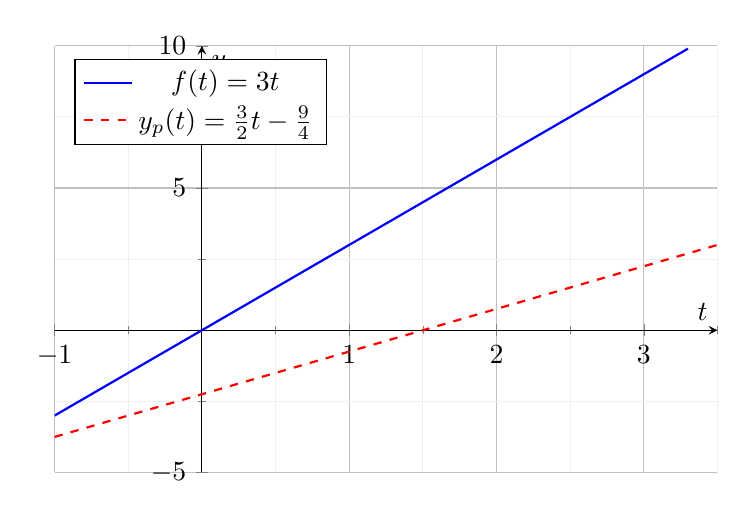
\begin{tikzpicture}
        \begin{axis}[
            axis lines = middle,
            xlabel = $t$,
            ylabel = {$y$},
            ymin=-5, ymax=10,
            xmin=-1, xmax=3.5,
            legend pos = north west,
            grid = both,
            minor tick num = 1,
            major grid style = {lightgray},
            minor grid style = {lightgray!25},
            width = 10cm,
            height = 7cm
        ]
        % Funcion forzadora f(t) = 3t
        \addplot[domain=-1:3.3, samples=100, color=blue, thick] {3*x};
        \addlegendentry{$f(t) = 3t$}

        % Solucion particular y_p(t) = 1.5t - 2.25
        \addplot[domain=-1:3.5, samples=100, color=red, thick, dashed] {1.5*x - 2.25};
        \addlegendentry{$y_p(t) = \frac{3}{2}t - \frac{9}{4}$}
        \end{axis}
    \end{tikzpicture}
    \caption{La funci\'on forzadora $f(t)$ (azul) y la correspondiente soluci\'on particular $y_p(t)$ (rojo). N\'otese que la soluci\'on particular tiene la misma forma que la funci\'on forzadora: ambas son funciones lineales.}
    \label{fig:forzadora_vs_particular}
\end{figure}

\begin{remark}
    El ejemplo anterior sugiere que para ecuaciones del tipo
    \[
    ay''+by'+cy=Ct^m,
    \]
    tiene sentido buscar soluciones de la forma
    \[
    y_p(t)=A_mt^m+A_{m-1}t^{m-1}+\cdots+A_1t+A_0,
    \]
    siempre que $c\neq 0$ (es decir, que $r=0$ no sea ra\'iz de la ecuaci\'on auxiliar; el caso contrario lo trataremos m\'as adelante). Lo que debemos hacer es encontrar los coeficientes $A_i$ y, tal como en el ejemplo anterior, para ello debemos resolver un sistema de $m+1$ ecuaciones con $m+1$ inc\'ognitas. Es por esto que a este m\'etodo lo llamaremos de los \textbf{coeficientes indeterminados}.
\end{remark}

\begin{example}
    Determinemos una soluci\'on particular de la ecuaci\'on:
    \[
    y''+3y'+2y=10e^{3t}.
    \]
    En este caso supondremos que la funci\'on que buscamos es de la forma $y(t)=Ae^{3t}$, con lo cual, si reemplazamos:
    \[
    9Ae^{3t}+3(3Ae^{3t})+2(Ae^{3t})=10e^{3t}\Longrightarrow 20Ae^{3t}=10e^{3t}.
    \]
    De aqu\'i $A=\dfrac{1}{2}$, con lo cual nuestra soluci\'on es
    \[
    y_p(t)=\dfrac{1}{2}e^{3t}.
    \]
\end{example}

Continuemos con el siguiente ejemplo.

\begin{example}
    Determinemos una soluci\'on particular de la ecuaci\'on
    \[
    y''+3y'+2y=\sin(t).
    \]
    Aqu\'i es natural que nuestra apuesta inicial sea una funci\'on del tipo $y(t)=A\sin(t)$, pero r\'apidamente nos daremos cuenta de que al derivarla aparece $\cos(t)$. Como las derivadas de $\sin(t)$ y $\cos(t)$ se transforman una en la otra, es razonable suponer que la soluci\'on que buscamos es del tipo
    \[
    y_p(t)=A\sin(t)+B\cos(t).
    \]
    Con esto en mente, reemplazamos en la ecuaci\'on:
    \[
    \big(-A\sin(t)-B\cos(t)\big)+3\big(A\cos(t)-B\sin(t)\big)+2\big(A\sin(t)+B\cos(t)\big)=\sin(t),
    \]
    es decir,
    \[
    (A-3B)\sin(t)+(3A+B)\cos(t)=\sin(t).
    \]
    Igualando coeficientes obtenemos
    \begin{align*}
        A-3B&=1,\\
        3A+B&=0,
    \end{align*}
    de donde $A=\dfrac{1}{10}$, $B=-\dfrac{3}{10}$. Con lo cual nuestra soluci\'on particular es:
    \[
    y_p(t)=\dfrac{1}{10}\sin(t)-\dfrac{3}{10}\cos(t).
    \]
\end{example}

\begin{remark}
    De manera m\'as general, dada una ecuaci\'on del tipo
    \[
    ay''+by'+cy=k\sin(\beta t)\quad \text{o bien}\quad ay''+by'+cy=k\cos(\beta t),
    \]
    el \textbf{m\'etodo de los coeficientes indeterminados} propone buscar soluciones de la forma
    \[
    y_p(t)=A\cos(\beta t)+B\sin(\beta t),
    \]
    siempre que $i\beta$ no sea ra\'iz de la ecuaci\'on auxiliar. Notemos que, aunque el lado derecho tenga solo un seno (o solo un coseno), la soluci\'on propuesta debe incluir ambas funciones.
\end{remark}

\begin{figure}[h!]
    \centering
    \begin{subfigure}[b]{0.32\textwidth}
        \centering
        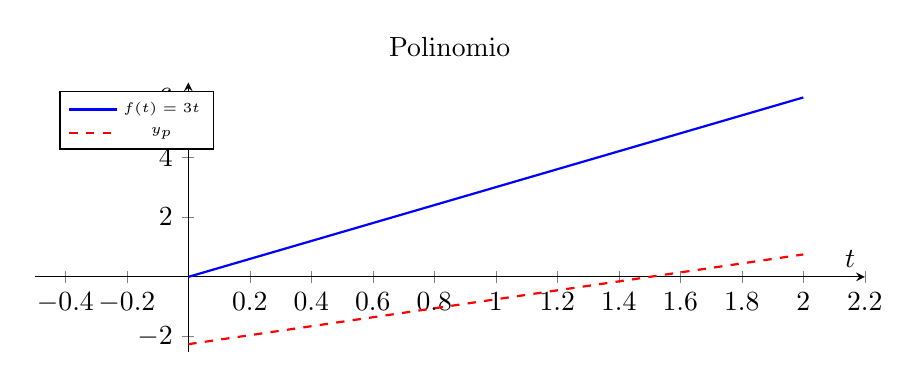
\begin{tikzpicture}
            \begin{axis}[
                axis lines = middle,
                xlabel = $t$, ylabel = {$y$},
                ymin=-2.5, ymax=6.5, xmin=-0.5, xmax=2.2,
                title = {Polinomio},
                width=\textwidth, height=5cm,
                legend pos = north west,
                legend style={font=\tiny}
            ]
            \addplot[domain=0:2, samples=50, blue, thick] {3*x};
            \addlegendentry{$f(t)=3t$}
            \addplot[domain=0:2, samples=50, red, thick, dashed] {1.5*x - 2.25};
            \addlegendentry{$y_p$}
            \end{axis}
        \end{tikzpicture}
    \end{subfigure}
    \hfill
    \begin{subfigure}[b]{0.32\textwidth}
        \centering
        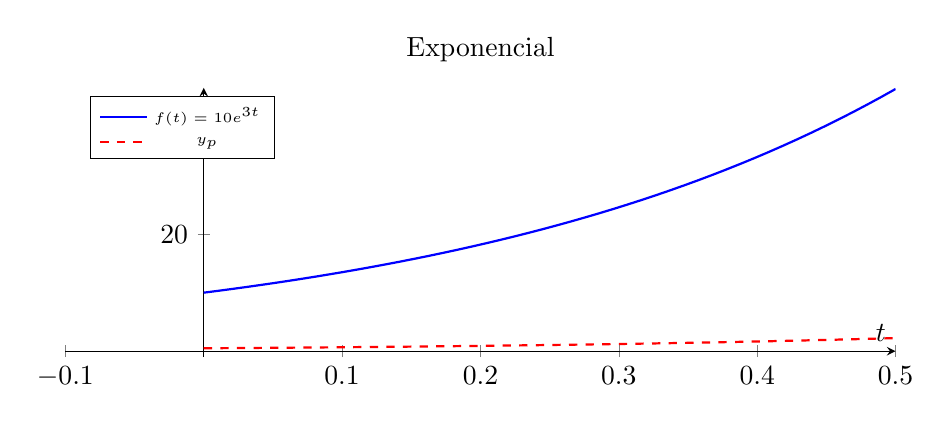
\begin{tikzpicture}
            \begin{axis}[
                axis lines = middle,
                xlabel = $t$, ylabel = {$y$},
                ymin=-1, ymax=45, xmin=-0.1, xmax=0.5,
                title = {Exponencial},
                width=\textwidth, height=5cm,
                legend pos = north west,
                legend style={font=\tiny}
            ]
            \addplot[domain=0:0.5, samples=50, blue, thick] {10*exp(3*x)};
            \addlegendentry{$f(t)=10e^{3t}$}
            \addplot[domain=0:0.5, samples=50, red, thick, dashed] {0.5*exp(3*x)};
            \addlegendentry{$y_p$}
            \end{axis}
        \end{tikzpicture}
    \end{subfigure}
    \hfill
    \begin{subfigure}[b]{0.32\textwidth}
        \centering
        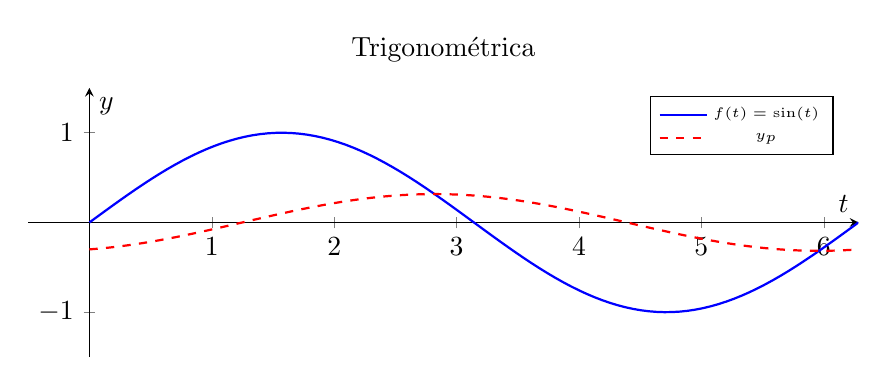
\begin{tikzpicture}
            \begin{axis}[
                axis lines = middle,
                xlabel = $t$, ylabel = {$y$},
                ymin=-1.5, ymax=1.5, xmin=-0.5, xmax=2*pi,
                title = {Trigonom\'etrica},
                width=\textwidth, height=5cm,
                legend pos = north east,
                legend style={font=\tiny}
            ]
            \addplot[domain=0:2*pi, samples=100, blue, thick] {sin(deg(x))};
            \addlegendentry{$f(t)=\sin(t)$}
            \addplot[domain=0:2*pi, samples=100, red, thick, dashed] {0.1*sin(deg(x)) - 0.3*cos(deg(x))};
            \addlegendentry{$y_p$}
            \end{axis}
        \end{tikzpicture}
    \end{subfigure}
    \caption{Ejemplos del m\'etodo de coeficientes indeterminados para diferentes tipos de funciones forzadoras. La soluci\'on particular $y_p$ (rojo) tiene una forma similar a la funci\'on forzadora $f(t)$ (azul).}
    \label{fig:coeficientes_indeterminados}
\end{figure}

A continuaci\'on comenzaremos a complicarnos un poco la vida.

\begin{example}
    Determinemos una soluci\'on particular de la ecuaci\'on:
    \[
    y''+4y=5t^2e^t.
    \]
    En vista de los ejemplos anteriores, en este caso buscaremos una soluci\'on del tipo
    \[
    y_p(t)=(At^2+Bt+C)e^{t},
    \]
    la cual, al reemplazarla en la ecuaci\'on dada, nos conduce a:
    \[
    e^t(2A+2B+C+4C)+te^t(4A+B+4B)+t^2e^t(A+4A)=5t^2e^t.
    \]
    Igualando coeficientes obtenemos el sistema
    \[
    5A=5,\qquad 4A+5B=0,\qquad 2A+2B+5C=0,
    \]
    cuya soluci\'on es $A=1$, $B=-\dfrac{4}{5}$, $C=-\dfrac{2}{25}$. Con lo cual la soluci\'on buscada es:
    \[
    y_p(t)=\left(t^2-\dfrac{4}{5}t-\dfrac{2}{25}\right)e^t.
    \]
\end{example}

\begin{remark}[\textquestiondown Por qu\'e funciona el m\'etodo?]
    En todos los ejemplos anteriores, la funci\'on $f(t)$ pertenece a una familia que es \emph{cerrada bajo derivaci\'on}: al derivar un polinomio se obtiene otro polinomio, al derivar $e^{rt}$ se obtiene un m\'ultiplo de $e^{rt}$, y al derivar senos y cosenos se obtienen senos y cosenos. Por eso, al reemplazar la forma propuesta en la ecuaci\'on no aparecen funciones nuevas, y basta igualar coeficientes.

    Esto tambi\'en explica las limitaciones del m\'etodo: para funciones como $\tan(t)$, $\ln(t)$ o $\dfrac{1}{t}$, cada derivada produce funciones nuevas, y no existe una forma finita que proponer. Para esos casos necesitaremos otro m\'etodo: la \textbf{variaci\'on de par\'ametros}, que estudiaremos en la siguiente secci\'on.
\end{remark}

Parece que nuestro m\'etodo escala bastante bien con problemas de complejidad mayor, pero (siempre hay alg\'un pero) consideremos la siguiente ecuaci\'on:
\[
y''-6y'+9y=e^{3t}.
\]
En este caso, la soluci\'on propuesta $y_p(t)=Ae^{3t}$, una vez reemplazada en la ecuaci\'on, nos conduce a:
\[
(Ae^{3t})''-6(Ae^{3t})'+9(Ae^{3t})=9Ae^{3t}-18Ae^{3t}+9Ae^{3t}=0,
\]
por lo tanto deber\'iamos tener $0=e^{3t}$, lo cual es claramente una contradicci\'on.

Lo que sucede en este caso es que la ecuaci\'on homog\'enea $y''-6y'+9y=0$ tiene por ecuaci\'on auxiliar $r^2-6r+9=(r-3)^2=0$, la cual tiene a $r=3$ como ra\'iz doble. Es decir, $e^{3t}$ \emph{ya es soluci\'on de la ecuaci\'on homog\'enea}, y por eso al reemplazarla el lado izquierdo se anula. Por la misma raz\'on, si intentamos con $y_p(t)=Ate^{3t}$ tampoco obtendremos soluci\'on, pues $te^{3t}$ tambi\'en es soluci\'on de la homog\'enea.

En este ejemplo debemos buscar una soluci\'on del tipo $y_p(t)=At^2e^{3t}$. En efecto,
\[
y_p'=A(2t+3t^2)e^{3t},\qquad y_p''=A(2+12t+9t^2)e^{3t},
\]
y al reemplazar,
\[
y_p''-6y_p'+9y_p=Ae^{3t}\big[(2+12t+9t^2)-6(2t+3t^2)+9t^2\big]=2Ae^{3t}=e^{3t},
\]
de donde $A=\dfrac{1}{2}$. Luego $y_p(t)=\dfrac{1}{2}t^2e^{3t}$ es una soluci\'on particular de la ecuaci\'on planteada.

\begin{figure}[h!]
    \centering
    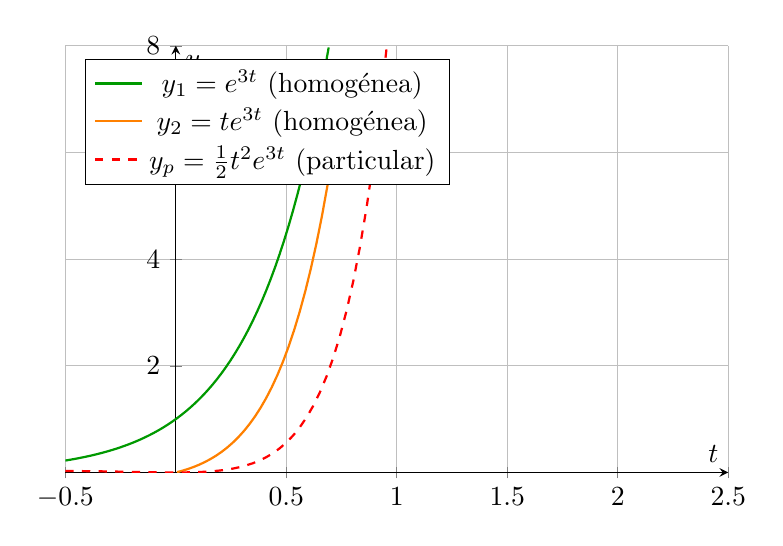
\begin{tikzpicture}
        \begin{axis}[
            axis lines = middle,
            xlabel = $t$,
            ylabel = {$y$},
            ymin=0, ymax=8,
            xmin=-0.5, xmax=2.5,
            restrict y to domain=0:8,
            legend pos = north west,
            grid = both,
            width = 10cm,
            height = 7cm
        ]
        % Solucion homogenea e^(3t)
        \addplot[domain=-0.5:1.5, samples=100, color=green!60!black, thick] {exp(3*x)};
        \addlegendentry{$y_1 = e^{3t}$ (homog\'enea)}

        % Solucion homogenea t*e^(3t)
        \addplot[domain=-0.5:2, samples=100, color=orange, thick] {x*exp(3*x)};
        \addlegendentry{$y_2 = te^{3t}$ (homog\'enea)}

        % Solucion particular t^2*e^(3t)
        \addplot[domain=-0.5:2.5, samples=100, color=red, thick, dashed] {0.5*x^2*exp(3*x)};
        \addlegendentry{$y_p = \frac{1}{2}t^2e^{3t}$ (particular)}
        \end{axis}
    \end{tikzpicture}
    \caption{Coincidencia con la soluci\'on homog\'enea. Las funciones $e^{3t}$ y $te^{3t}$ son soluciones de la ecuaci\'on homog\'enea (curvas verde y naranja). Como la funci\'on forzadora $e^{3t}$ coincide con una soluci\'on homog\'enea, es necesario multiplicar por $t^2$ para encontrar una soluci\'on particular (curva roja discontinua).}
    \label{fig:coincidencia}
\end{figure}

El mismo fen\'omeno aparece con funciones trigonom\'etricas, y en ese caso tiene una interpretaci\'on f\'isica muy importante.

\begin{example}[Resonancia]
    Consideremos la ecuaci\'on
    \[
    y''+y=\cos(t),
    \]
    que modela un sistema masa-resorte \emph{sin amortiguaci\'on}, cuya frecuencia natural es $1$, sometido a una fuerza externa que oscila con esa misma frecuencia. La ecuaci\'on auxiliar $r^2+1=0$ tiene ra\'ices $\pm i$, as\'i que $\cos(t)$ y $\sin(t)$ son soluciones de la homog\'enea, y la forma $A\cos(t)+B\sin(t)$ no sirve. Proponemos entonces
    \[
    y_p(t)=t\big(A\cos(t)+B\sin(t)\big).
    \]
    Derivando,
    \begin{align*}
        y_p'&=A\cos(t)+B\sin(t)+t\big(-A\sin(t)+B\cos(t)\big),\\
        y_p''&=-2A\sin(t)+2B\cos(t)-t\big(A\cos(t)+B\sin(t)\big),
    \end{align*}
    y al reemplazar, los t\'erminos con $t$ se cancelan:
    \[
    y_p''+y_p=-2A\sin(t)+2B\cos(t)=\cos(t),
    \]
    de donde $A=0$, $B=\dfrac{1}{2}$. As\'i,
    \[
    y_p(t)=\dfrac{t}{2}\sin(t).
    \]
    El factor $t$ hace que la amplitud de la oscilaci\'on crezca sin l\'imite: este fen\'omeno se conoce como \textbf{resonancia}, y es el responsable, por ejemplo, de que una copa de cristal pueda romperse con una nota musical de la frecuencia adecuada.
\end{example}

\begin{figure}[h!]
    \centering
    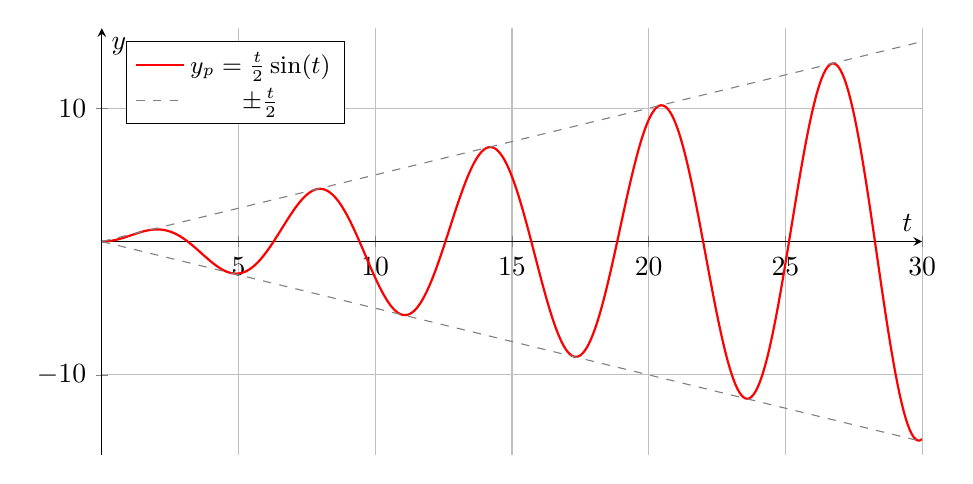
\begin{tikzpicture}
        \begin{axis}[
            axis lines = middle,
            xlabel = $t$,
            ylabel = {$y$},
            ymin=-16, ymax=16,
            xmin=0, xmax=30,
            legend pos = north west,
            legend style={font=\small},
            grid = both,
            width = 12cm,
            height = 7cm
        ]
        \addplot[domain=0:30, samples=400, color=red, thick] {0.5*x*sin(deg(x))};
        \addlegendentry{$y_p=\frac{t}{2}\sin(t)$}
        \addplot[domain=0:30, samples=2, color=gray, dashed] {0.5*x};
        \addlegendentry{$\pm\frac{t}{2}$}
        \addplot[domain=0:30, samples=2, color=gray, dashed, forget plot] {-0.5*x};
        \end{axis}
    \end{tikzpicture}
    \caption{Resonancia: cuando la frecuencia de la fuerza externa coincide con la frecuencia natural del sistema, la amplitud de las oscilaciones crece linealmente con el tiempo.}
    \label{fig:resonancia}
\end{figure}

De manera general, podemos resumir el m\'etodo desarrollado hasta el momento con el siguiente resultado.

\begin{theorem}
    Para encontrar una soluci\'on particular de la ecuaci\'on
    \[
    ay''+by'+cy=Ct^me^{rt},
    \]
    donde $m$ es un entero no negativo, existe una soluci\'on particular de la forma
    \[
    y_p(t)=t^{s}\left(A_mt^m+\cdots+A_1t+A_0\right)e^{rt},
    \]
    donde
    \begin{enumerate}[label=\roman*)]
        \item $s=0$ si $r$ no es ra\'iz de la ecuaci\'on auxiliar,
        \item $s=1$ si $r$ es una ra\'iz simple de la ecuaci\'on auxiliar,
        \item $s=2$ si $r$ es una ra\'iz doble de la ecuaci\'on auxiliar.
    \end{enumerate}

    Para el caso en que la ecuaci\'on sea del tipo
    \[
    ay''+by'+cy=Ct^me^{\alpha t}\cos(\beta t)\quad \text{o bien}\quad ay''+by'+cy=Ct^me^{\alpha t}\sin(\beta t),
    \]
    con $\beta\neq 0$, existe una soluci\'on particular de la forma
    \[
    y_p(t)=t^s\left(A_mt^m+\cdots+A_0\right)e^{\alpha t}\cos(\beta t)+t^s\left(B_mt^m+\cdots+B_0\right)e^{\alpha t}\sin(\beta t),
    \]
    donde
    \begin{enumerate}[label=\roman*),resume]
        \item $s=0$ si $\alpha+i\beta$ no es ra\'iz de la ecuaci\'on auxiliar,
        \item $s=1$ si $\alpha+i\beta$ es ra\'iz de la ecuaci\'on auxiliar.
    \end{enumerate}
\end{theorem}

Notemos que el caso $s=2$ no aparece en la segunda parte: como los coeficientes $a,b,c$ son reales, una ra\'iz compleja $\alpha+i\beta$ con $\beta\neq0$ siempre es simple (su conjugada $\alpha-i\beta$ es la otra ra\'iz). El ejemplo $y''-6y'+9y=e^{3t}$ corresponde al caso iii), y el ejemplo de resonancia al caso v), con $\alpha=0$, $\beta=1$.

En la pr\'actica resulta \'util tener a mano la siguiente tabla, donde $P_m(t)$ denota un polinomio de grado $m$. La forma indicada se multiplica luego por $t^s$ seg\'un el teorema anterior.

\begin{center}
\small\renewcommand{\arraystretch}{1.6}
\begin{tabular}{|c|c|}
\hline
$f(t)$ & \textbf{Forma de} $y_p$ \\ \hline
$P_m(t)$ & $A_mt^m+\cdots+A_0$ \\ \hline
$e^{rt}$ & $Ae^{rt}$ \\ \hline
$\cos(\beta t)$ o $\sin(\beta t)$ & $A\cos(\beta t)+B\sin(\beta t)$ \\ \hline
$P_m(t)e^{rt}$ & $(A_mt^m+\cdots+A_0)e^{rt}$ \\ \hline
$P_m(t)e^{\alpha t}\cos(\beta t)$ o $\sin(\beta t)$ & $e^{\alpha t}\left[(A_mt^m+\cdots+A_0)\cos(\beta t)+(B_mt^m+\cdots+B_0)\sin(\beta t)\right]$ \\ \hline
\end{tabular}
\end{center}

Hay ocasiones en las cuales es necesario resolver ecuaciones del tipo
\[
y''+3y'+2y=3t+10e^{3t}+\sin(t),
\]
y claramente no queremos buscar una soluci\'on en la cual ser\'ia necesario determinar $5$ coeficientes de manera simult\'anea. En estos casos contamos con la siguiente propiedad, que generaliza el \textbf{principio de superposici\'on} de la secci\'on anterior al caso no homog\'eneo.

\begin{remark}[Principio de superposici\'on]
    Sea $y_1$ una soluci\'on de la ecuaci\'on diferencial
    \[
    ay''+by'+cy=f_1(t),
    \]
    y sea $y_2$ una soluci\'on de la ecuaci\'on
    \[
    ay''+by'+cy=f_2(t).
    \]
    Entonces, para todo par de constantes reales $k_1,k_2$, la funci\'on $y(t)=k_1y_1(t)+k_2y_2(t)$ es soluci\'on de la ecuaci\'on
    \[
    ay''+by'+cy=k_1f_1(t)+k_2f_2(t).
    \]
    En particular, con $k_1=k_2=1$, la suma $y_1+y_2$ es soluci\'on de la ecuaci\'on con lado derecho $f_1+f_2$.
\end{remark}

\begin{example}
    Sabemos, de los ejemplos anteriores, que $y_1(t)=\dfrac{3}{2}t-\dfrac{9}{4}$ es soluci\'on de
    \[
    y''+3y'+2y=3t,
    \]
    y que $y_2(t)=\dfrac{1}{2}e^{3t}$ es soluci\'on de
    \[
    y''+3y'+2y=10e^{3t}.
    \]
    Luego, en vista del resultado anterior, una soluci\'on particular de la ecuaci\'on
    \[
    y''+3y'+2y=3t+10e^{3t}
    \]
    es $y_p(t)=\dfrac{3}{2}t-\dfrac{9}{4}+\dfrac{1}{2}e^{3t}$.

    Del mismo modo, como $y_3(t)=\dfrac{1}{10}\sin(t)-\dfrac{3}{10}\cos(t)$ es soluci\'on de $y''+3y'+2y=\sin(t)$, la ecuaci\'on con la que motivamos esta propiedad,
    \[
    y''+3y'+2y=3t+10e^{3t}+\sin(t),
    \]
    tiene por soluci\'on particular
    \[
    y_p(t)=\dfrac{3}{2}t-\dfrac{9}{4}+\dfrac{1}{2}e^{3t}+\dfrac{1}{10}\sin(t)-\dfrac{3}{10}\cos(t),
    \]
    sin necesidad de resolver un sistema de $5\times 5$.
\end{example}

\begin{figure}[h!]
    \centering
    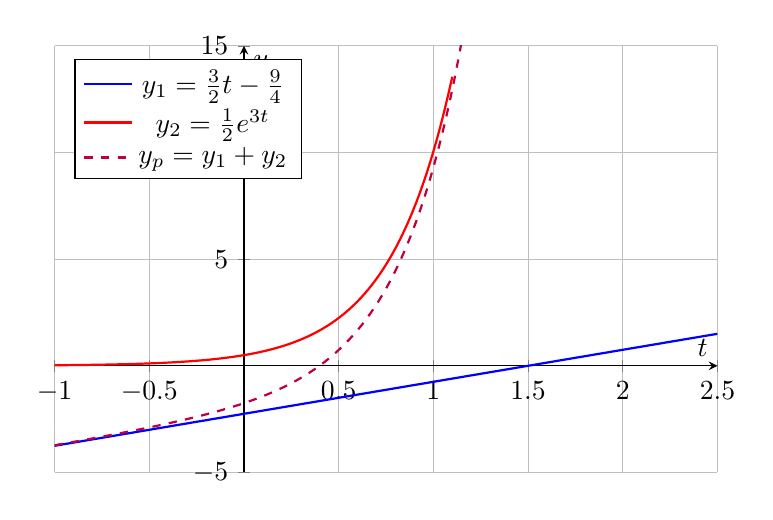
\begin{tikzpicture}
        \begin{axis}[
            axis lines = middle,
            xlabel = $t$,
            ylabel = {$y$},
            ymin=-5, ymax=15,
            xmin=-1, xmax=2.5,
            legend pos = north west,
            grid = both,
            width = 10cm,
            height = 7cm
        ]
        % y1(t) = 1.5t - 2.25
        \addplot[domain=-1:2.5, samples=100, color=blue, thick] {1.5*x - 2.25};
        \addlegendentry{$y_1 = \frac{3}{2}t - \frac{9}{4}$}

        % y2(t) = 0.5*e^(3t)
        \addplot[domain=-1:1.1, samples=100, color=red, thick] {0.5*exp(3*x)};
        \addlegendentry{$y_2 = \frac{1}{2}e^{3t}$}

        % y1 + y2
        \addplot[domain=-1:1.2, samples=100, color=purple, thick, dashed] {1.5*x - 2.25 + 0.5*exp(3*x)};
        \addlegendentry{$y_p = y_1 + y_2$}
        \end{axis}
    \end{tikzpicture}
    \caption{El principio de superposici\'on. La soluci\'on particular para la suma de dos funciones forzadoras, $3t+10e^{3t}$, es la suma de las soluciones particulares individuales.}
    \label{fig:superposicion}
\end{figure}

El siguiente resultado es la extensi\'on del \textbf{teorema de existencia y unicidad} al caso de ecuaciones no homog\'eneas.

\begin{theorem}
    Sean $a\neq 0$ y $y_1(t),y_2(t)$ dos soluciones linealmente independientes de la ecuaci\'on
    \[
    ay''+by'+cy=0,
    \]
    y sea $y_p(t)$ una soluci\'on particular de la ecuaci\'on
    \[
    ay''+by'+cy=f(t).
    \]
    Entonces el problema de valor inicial
    \[
    ay''+by'+cy=f(t), \qquad y(t_0)=Y_0,\qquad y'(t_0)=Y_1,
    \]
    admite una \'unica soluci\'on, y esta es de la forma
    \[
    y(t)=c_1y_1(t)+c_2y_2(t)+y_p(t),
    \]
    para una adecuada elecci\'on de constantes $c_1,c_2\in \mathbb{R}$.
\end{theorem}

\begin{example}
    Consideremos el PVI dado por
    \[
    y''-y=2-t^2,\qquad y(0)=1,\qquad y'(0)=0.
    \]
    En primer lugar determinamos la soluci\'on de la respectiva ecuaci\'on homog\'enea. Esta tiene ecuaci\'on auxiliar $r^2-1=0$, con ra\'ices $r=\pm1$, con lo cual:
    \[
    y_h=c_1e^t+c_2e^{-t}.
    \]
    Por otro lado, como $r=0$ no es ra\'iz de la ecuaci\'on auxiliar, buscamos una soluci\'on particular de la forma $y_p(t)=A+Bt+Ct^2$. Como $y_p''=2C$, al reemplazar obtenemos
    \[
    2C-(A+Bt+Ct^2)=2-t^2\Longrightarrow -Ct^2-Bt+(2C-A)=-t^2+2,
    \]
    de donde $C=1$, $B=0$ y $2C-A=2$, es decir, $A=0$. Luego $y_p(t)=t^2$, y la soluci\'on general es
    \[
    y(t)=c_1e^t+c_2e^{-t}+t^2.
    \]
    Imponiendo las condiciones iniciales:
    \[
    y(0)=c_1+c_2=1,\qquad y'(0)=c_1-c_2=0,
    \]
    encontramos que $c_1=c_2=\dfrac{1}{2}$, es decir, la soluci\'on del PVI dado es:
    \[
    y(t)=t^2+\dfrac{1}{2}\left(e^t+e^{-t}\right)=t^2+\cosh(t).
    \]
\end{example}

Cerramos esta secci\'on proponiendo un problema a resolver.

\begin{exercise}
    Un sistema masa-resorte recibe una fuerza externa dada por $f(t)=5\sin(t)+5\cos(t)$. La masa es de $1\,\mathrm{kg}$, la constante del resorte es $k=2\,\mathrm{N/m}$ y el coeficiente de amortiguaci\'on del sistema es $b=2\,\mathrm{N\cdot s/m}$. Si la masa se encuentra, al inicio, un metro a la derecha de la posici\'on de equilibrio, con una velocidad de $2\,\mathrm{m/s}$, determine la posici\'on de la masa en el instante $t$.

    Compare su resultado con el gr\'afico de la Figura~\ref{fig:grafica_masa_resorte}.
\end{exercise}

\begin{figure}[h!]
    \centering
    \begin{tikzpicture}[
        every node/.style={font=\small}
    ]
        % --- Pared ---
        \draw[thick] (0,0) -- (0,3);
        \draw[pattern=north east lines, pattern color=black!60]
            (0,0) rectangle (0.2,3);

        % --- Resorte ---
        \draw[thick, decorate, decoration={zigzag, segment length=4mm, amplitude=2mm}]
            (0.2,2.5) -- (3,2.5);

        % --- Amortiguador (cilindro + piston) ---
        \draw[thick, fill=white] (0.2,1.35) rectangle (1.6,1.65);
        \draw[thick] (1.6,1.5) -- (3,1.5);
        \draw[thick] (1.6,1.35) -- (1.6,1.65);

        % --- Masa ---
        \draw[fill=gray!50] (3,0.8) rectangle (4,2.2);
        \node at (3.5,1.5) {$m=1$};

        % --- Fuerza externa ---
     \draw[{->}, thick, blue] (4,1.5) -- (5.5,1.5)
    node[right] {$f(t)$};

        % --- Etiquetas ---
        \node at (1.5,2.85) {$k=2$};
        \node at (1.0,1.0) {$b=2$};
    \end{tikzpicture}
    \caption{Diagrama del sistema masa-resorte-amortiguador con una fuerza externa $f(t)$.}
    \label{fig:sistema_masa_resorte}
\end{figure}

\begin{figure}[h!]
    \centering
    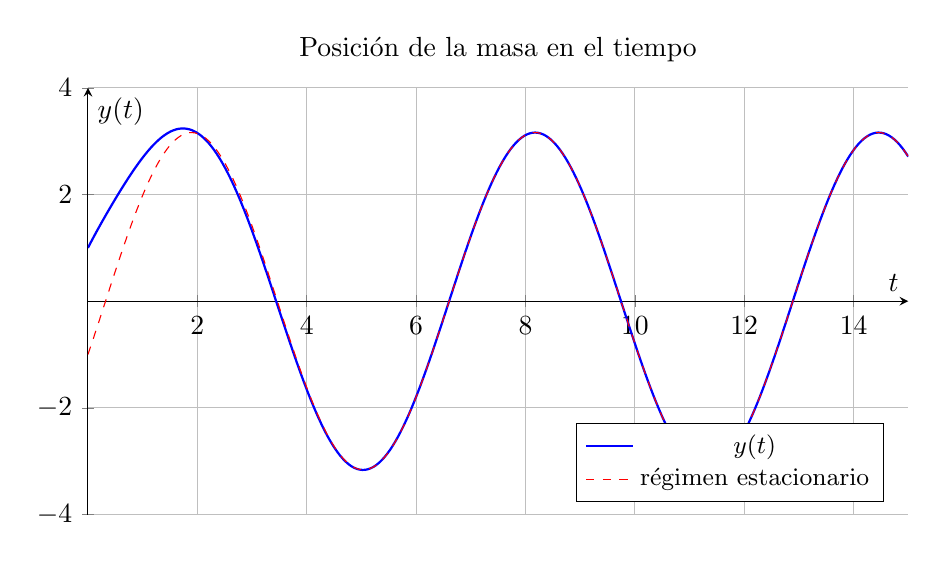
\begin{tikzpicture}
        \begin{axis}[
            axis lines = middle,
            xlabel = $t$,
            ylabel = {$y(t)$},
            ymin=-4, ymax=4,
            xmin=0, xmax=15,
            grid = both,
            legend pos = south east,
            legend style={font=\small},
            width = 12cm,
            height = 7cm,
            title = {Posici\'on de la masa en el tiempo}
        ]
        % Solucion del PVI
        \addplot[domain=0:15, samples=300, color=blue, thick]
            {exp(-x)*(2*cos(deg(x)) + sin(deg(x))) - cos(deg(x)) + 3*sin(deg(x))};
        \addlegendentry{$y(t)$}
        % Regimen estacionario (solucion particular)
        \addplot[domain=0:15, samples=300, color=red, dashed]
            {-cos(deg(x)) + 3*sin(deg(x))};
        \addlegendentry{r\'egimen estacionario}
        \end{axis}
    \end{tikzpicture}
    \caption{Posici\'on de la masa en el tiempo (azul). Se observa un comportamiento transitorio que decae r\'apidamente, tras el cual la soluci\'on se confunde con el r\'egimen estacionario (rojo discontinuo), que es la soluci\'on particular debida a la fuerza externa.}
    \label{fig:grafica_masa_resorte}
\end{figure}
